\documentclass[twocolumn]{aastex631}
\received{\today}
\shorttitle{Giant Planet Formation}
\graphicspath{{figures/}}

\usepackage{lipsum}
\usepackage{physics}
\usepackage{multirow}
\usepackage{xspace}
\usepackage{natbib}
\usepackage{fontawesome5}
\usepackage{xcolor}
\usepackage{wrapfig}
\usepackage[figuresright]{rotating}

% remove indents in footnotes
\usepackage[hang,flushmargin]{footmisc} 

\newcommand{\todo}[1]{{\color{red}{[TODO: #1}]}}
\newcommand{\needcite}{{\color{magenta}{(needs citation)}}}
\newcommand{\placeholder}[1]{{\color{gray} \lipsum[#1]}}

% custom function for adding units
\makeatletter
\newcommand{\unit}[1]{%
    \,\mathrm{#1}\checknextarg}
\newcommand{\checknextarg}{\@ifnextchar\bgroup{\gobblenextarg}{}}
\newcommand{\gobblenextarg}[1]{\,\mathrm{#1}\@ifnextchar\bgroup{\gobblenextarg}{}}
\makeatother

\begin{document}

\title{{\huge Giant Planet Formation}\\\vspace{0.15cm}ASTR558 Final Project}

% affiliations
\newcommand{\UW}{Department of Astronomy, University of Washington, Seattle, WA, 98195}

\author[0000-0001-6147-5761]{Tom Wagg}
\affiliation{\UW}

\correspondingauthor{Tom Wagg}
\email{tomwagg@uw.edu}

\begin{abstract}
    There are currently two main theories for the formation of giant planets, core accretion and direct collapse. Core accretion can explain the formation of most planets but for those far from their host star, direct collapse is needed to explain their existence on the timescale of the age of the Universe. In this paper we explain the processes involved in each theory as well as their relative merits and limitations. We additionally discuss recent work in the field and highlight some major unsolved questions.
    \placeholder{1}
\end{abstract}

\keywords{}

\section{Key Concepts}

In this section, we explain the key concepts behind the two main theories of giant planet formation. Figure~\ref{fig:formation_diagram} provides a schematic illustration of the two formation channels that we discuss.

\subsection{Core Accretion}

\subsubsection{How does it work?}

At its simplest level, core accretion is where a central rocky core is formed and then accretes gas until it reaches a critical core mass and forms a giant planet \citep{Pollack+1996}. This general process is illustrated in the left planet of Figure~\ref{fig:formation_diagram}.

The formation occurs in three phases, which can be seen in Figure~\ref{fig:planet_growth}. In the first phase, the planet is formed primarily of solid material and continuously accretes planetessimals at a higher rate than gas until the planet clears its ``feeding zone'', marking the end of the first phase. At this point the core of the planet has formed and now the planet slowly accretes gas in an envelope. This gas is accreted from a sphere of radius \citep{Bodenheimer+2013}
\begin{equation}
    R = \min \{ R_{\rm Bondi}, R_{\rm Hill} \}
\end{equation}
where $R_{\rm Bondi}$ is the Bondi radius, defining the maximum distance inside which gas can be bound to the core and $R_{\rm Hill}$ is the Hill radius, defining the radius in which the main gravitational influence is the planet. See Appendix~\ref{app:maths} for a derivation of these radii.

The third phase of core accretion begins as the planetary core exceeds the critical core mass, resulting in rapid envelope contraction that leads to fast accretion of gas and thus planet mass growth. This finals results in a giant planet.

\begin{figure}
    \centering
    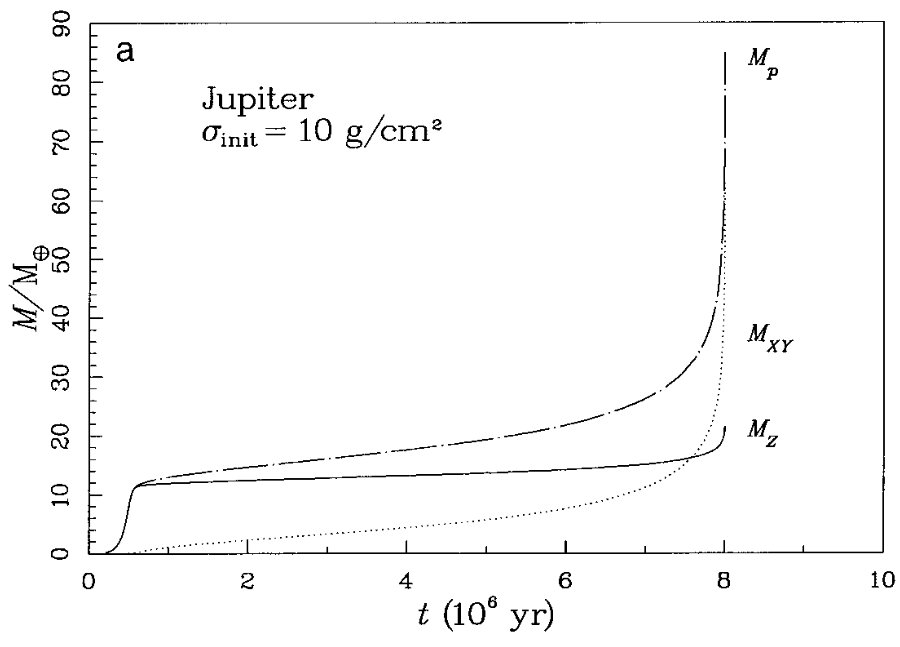
\includegraphics[width=\columnwidth]{pollack_fig_1.png}
    \caption{Figure 1 of \citet{Pollack+1996}. Planet mass as a function of time in which the three phases of core accretion are evident. Phase 1 is rapid early accretion of solids ($\sim$$0$--$0.4 \unit{Myr}$), Phase 2 is slow accretion onto the core ($\sim$$0.4$--$7.5 \unit{Myr}$) and Phase 3 is rapid final accretion once the critical core mass is exceeded ($\sim$$7.5$--$8 \unit{Myr}$). The different curves show the masses of different compositions.}
    \label{fig:planet_growth}
\end{figure}

\subsubsection{Critical core mass}

During Phase 2 of formation via core accretion, slow accretion of gas and solids onto the core increases the envelope mass over time. For a given core mass, there exists an envelope mass above which hydrostatic equilibrium cannot be satisfied, which triggers the collapse of the envelope onto the core and the beginning of Phase 3.

This critical core mass can be derived using some basic assumptions about the locations of convective and radiative zones \citep{Stevenson+1982,Lissauer+2009}. Previous work assumed that the envelope was fully radiative but a more accurate assumption is that there is an innermost convective zone and outermost radiative zone. The combination of these zones gives that the critical core mass is simply
\begin{equation}
    M_{c} = \frac{1}{2} M
\end{equation}
implying that once the core mass accounts for half of the overall planet mass, rapid contraction will occur and Phase 3 of formation begins.

\subsubsection{The end of accretion}

A giant planet formed via core accretion will finish its formation once there is no gas left for accretion. This termination occurs once the gas in the surrounding protoplanetary disc is dispersed (mainly by photo-evaporation). Prior to this dispersal, the accretion of a planet can also stall once it forms a gap in the protoplanetary disc after the end of Phase 3. This means that you can form different sorts of planets depending on what phase of formation they were in once the the gas in the disc is dispersed.

\citet{Lissauer+2009} showed that Saturn's mass is around the maximum for disc-limited accretion, whereas Neptune and Uranus were slower to form and would still have been on Phase 2 when the gas in the disc dispersed. The final planet mass therefore clearly depends on the star (specifically how luminous and how quickly it evolves) in addition to the planet location, disc density and other initial planet properties.

\subsubsection{Timescale limits}

The timescale on which core accretion occurs is strongly dependent on the distance of the planet from its host star. This means that, if we assume that all planets are formed via core accretion, one would expect that at larger distances the planets' masses would decrease (since they have less time to accrete or even reach Phase 3).

However, this is not what is seen observationally. In Figure~\ref{fig:demographics} we show a distribution of detected planets, plotting their separation against mass. It is evident that there is an abundance of large mass-large separation planets that couldn't possibly have been formed via core accretion. This leads to the second theory of giant planet formation - direct collapse.

\begin{figure}[tb]
    \centering
    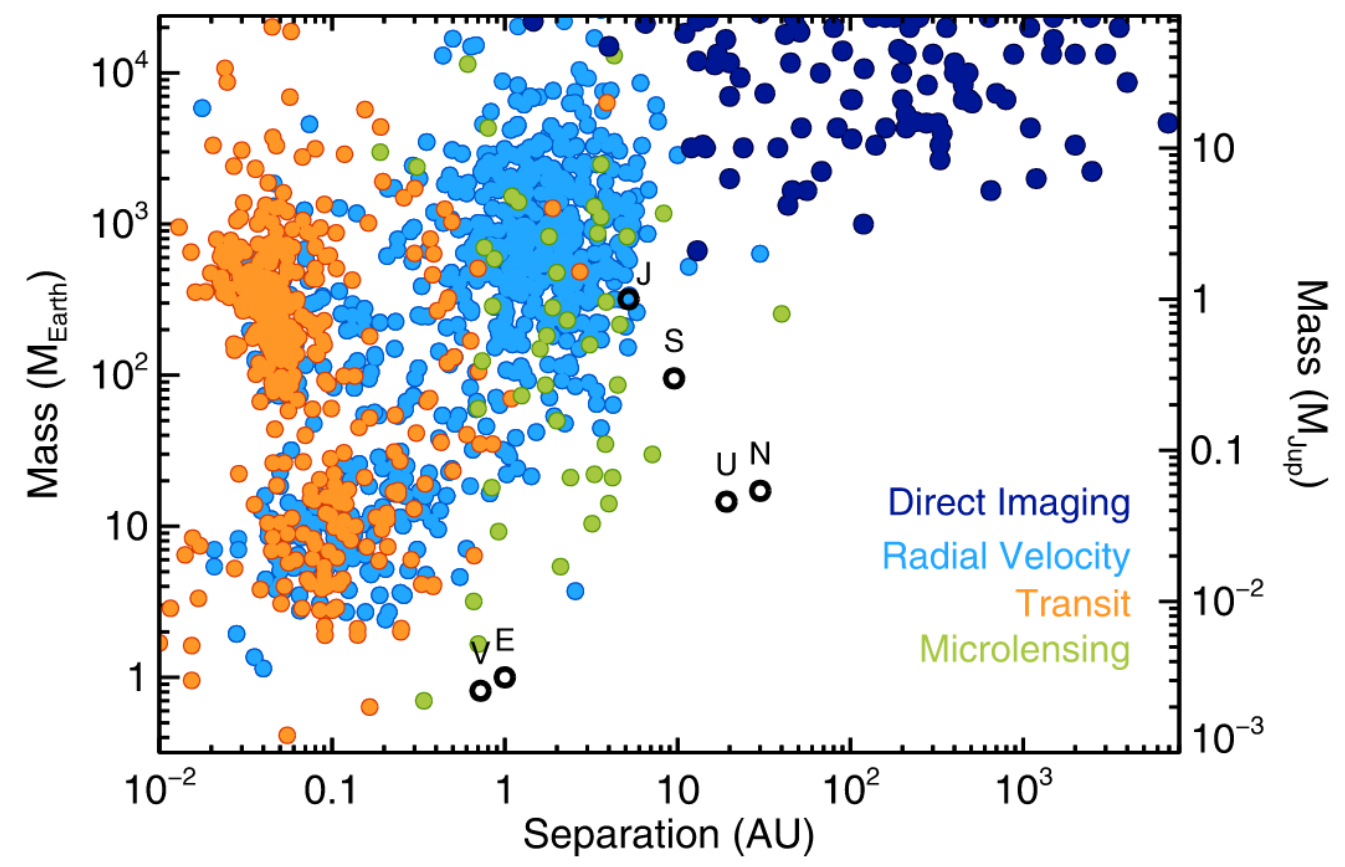
\includegraphics[width=\columnwidth]{exoplanet_demographics.png}
    \caption{Figure 13 from \citet{Bowler+2016}. Demographics of detected exoplanets, highlighting the large number of directly imaged planets that are far from their star whilst being very massive. These planets could not have been formed via core accretion.}
    \label{fig:demographics}
\end{figure}

\subsection{Direct Collapse}

\subsubsection{How does it work?}



\subsubsection{Migration}

\begin{figure}[b]
    \centering
    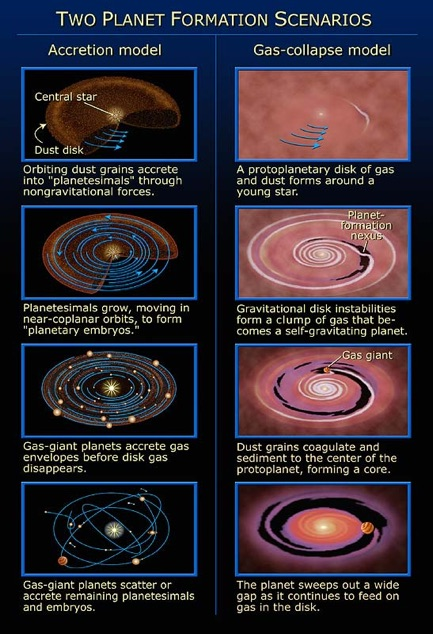
\includegraphics[width=\columnwidth]{channels_illustration.jpg}
    \caption{An illustration of different giant planet formation channels. (Credit: NASA and A. Feild (STScl))}
    \label{fig:formation_diagram}
\end{figure}

\section{Recent Research}

\section{Unsolved Questions}

\begin{itemize}
    \item Challenges with direct collapse \citep{Forgan+2013}
    \item Core accretion doesn't account for compositional gradients \citep{D'Angelo+2018}
\end{itemize}

\nocite{*}

\bibliographystyle{aasjournal}
\bibliography{paper}{}

\appendix

\section{Derivation of Bondi and Hill Radii}\label{app:maths}

\subsection{Bondi Radius}
The Bondi radius is the maximum distance inside which gas can be bound to the core of the planet. The gas will be bound to the core if, in the frame of the core, its total energy becomes negative. This means that the gravitational potential energy needs to be greater than the total thermal energy and so we can write
\begin{equation}
    \frac{G M_c}{R} \ge \frac{1}{2} (v_{\rm rel}^2 + v_{\rm th}^2),
\end{equation}
where $M_c$ is the core mass, $R$ is the radius, $v_{\rm rel}$ is the relative velocity of the gas and the core and $v_{\rm th}$ is the thermal velocity of the gas. If we assume that the relative velocity is dominated by Keplerian shear \citep{D'Angelo+2018} then
\begin{equation}
    \abs{v_{\rm rel}} = R \Omega,
\end{equation}
where $\Omega = \sqrt{G M_* / a^3}$ is the angular orbital velocity. And the thermal velocity is given by
\begin{equation}
    v_{\rm th} = c_g \sqrt{8 / \pi}
\end{equation}
where $c_g$ is the speed of sound in the gas. The sound speed is often expressed as $c_g = H_g \Omega$, where $H_g$ is the pressure scale height of the disc. We can now plug this all into the original inequality (and make it an inequality to solve for the Bondi radius)
\begin{align}
    \frac{G M_c}{R_{\rm B}} &= \frac{1}{2} (R^2 \Omega^2 + \frac{8}{\pi} H_g^2 \Omega^2) \\
    \frac{G M_c}{R_{\rm B}} &= \frac{G M_*}{2 a^3} (R^2 + \frac{8}{\pi} H_g^2) \\
    R_{\rm B} &= \frac{M_c}{M_*} \frac{2 a^3}{R^2 + \frac{8}{\pi} H_g^2} \\
    R_{\rm B} &= a \qty(\frac{M_c}{M_*}) \qty(\frac{a}{2 H_g})^2
\end{align}

\subsection{Hill Radius}
The Hill radius is a similar quantity but it is due to forces rather than energy. The radius is the maximum distance within which the main gravitational influence is the core of the planet. Let's assume a circular orbit in this case. Therefore, the Hill radius is found by equating the gravitational and centrifugal forces
\begin{equation}
    \frac{G M_p}{R_{\rm H}^2} - \frac{G M_*}{(a - R_{\rm H})^2} + \Omega (a - R_{\rm H}) = 0
\end{equation}
which we can equivalently write as follows using the definition of $\Omega$
\begin{equation}
    \frac{M_p}{R_{\rm H}^2} - \frac{M_*}{a^2} \qty(1 - \frac{R_{\rm H}}{a})^{-2} + \frac{M_*}{a^2} \qty(1 - \frac{R_{\rm H}}{a}) = 0
\end{equation}
Next we can take just the leading order to find
\begin{equation}
    \frac{M_p}{R_{\rm H}^2} - \frac{M_*}{a^2} \qty(1 + \frac{2 R_{\rm H}}{a}) + \frac{M_*}{a^2} \qty(1 - \frac{R_{\rm H}}{a}) = 0
\end{equation}
This gives the definition of the Hill radius as
\begin{equation}
    R_{\rm H} = a \qty(\frac{M_p}{3 M_*})^{1/3}
\end{equation}


\end{document}